\section{Methodology}
\label{sec:methodology}

We now present a brief description of the NDN model (...) for this work. We 
start (...).

\subsection{Overview}
\label{subsec:meth-overview}

We consider a conceptual NDN network composed by three main types of 
entities: (1) 
$|R|$ NDN routers\footnote{Here we use the notation $|E|$ to 
represent the number of elements of type $E$.} $R_r$, $r = \{1,2,...,|R|\}$, 
organized in some type of topology (e.g. cascade, tree, etc.); (2) a set of 
$|C|$ clients $C_c$, $c = \{1,2,...,|C|\}$; and a single 
content server $S$, holding $|O|$ different content objects $O_o$, 
$o = \{1,2,...,|O|\}$ (e.g. $|O|$ different photos).\shortvertbreak

Clients issue requests for content objects $O_o$, i.e. Interest packets $i_{O_o}$, which 
are propagated through NDN routers towards the content server $S$, and 
eventually followed by Data packets 
$d_{O_o}$, containing the requested content object. We represent the 
elementary set of signals fed to\slash read from the inputs\slash outputs of the 
aforementioned basic 
entities, at some discrete time instant $t$, as a $2\,|O| \times 1 $ array in the form

\begin{equation}
    \textbf{u}[t] = \begin{bmatrix}  i_{O_1}         \\ 
                            i_{O_2}         \\ 
                             ...            \\ 
                            i_{O_{|O|}}     \\ 
                            d_{O_1}         \\ 
                            d_{O_2}         \\ 
                             ...            \\ 
                            d_{O_{|O|}}     \\ \end{bmatrix}
    \label{eq:signal}
\end{equation}\shortvertbreak

Each component $i_{O_o}$ or $d_{O_o}$ may assume an integer value, i.e. $i_{O_o}, d_{O_o} \in \mathbb{N}_0 = \{0, 1, 2, ... \}$, 
representing the absence (in case of $i_{O_o}, d_{O_o} = 0$) or presence (in case of $i_{O_o}, d_{O_o} > 0$) of an 
Interest\slash Data packet, at a given time instant $t$. E.g. considering a setting 
with $|O| = 2$ content objects, a value of \textbf{u} corresponding to the presence 
of two Interests for content $O_1$ and one Data packet for $O_2$ (with the absence 
for the remaining components) would be encoded as

\begin{equation}
    \textbf{u}[t] = \begin{bmatrix}     2   \\ 
                                        0   \\ 
                                        0   \\ 
                                        1   \\ \end{bmatrix}
    \label{eq:signal-eg}
\end{equation}\shortvertbreak

With this 
representation of \textbf{u}, we capture situations in which a network 
entity may simultaneously receive\slash issue any Interest or Data packet as 
its input\slash output.

\subsection{NDN Router Model}
\label{subsec:meth-overview}

An NDN router is the central entity of the presented model, acting 
as the main agent of NDN's forwarding engine. It is also the more complex entity, 
including a set of submodules, already 
mentioned in Section~\ref{sec:ndn}: (1) the Forward Information Base (FIB); (2) 
the Pending Interest Table (PIT); and (3) the Content Store (CS). We first 
provide an overview of our NDN router module, and then proceed with the description 
of each one of its submodules.\shortvertbreak

\begin{figure}[h!]

    \centering
    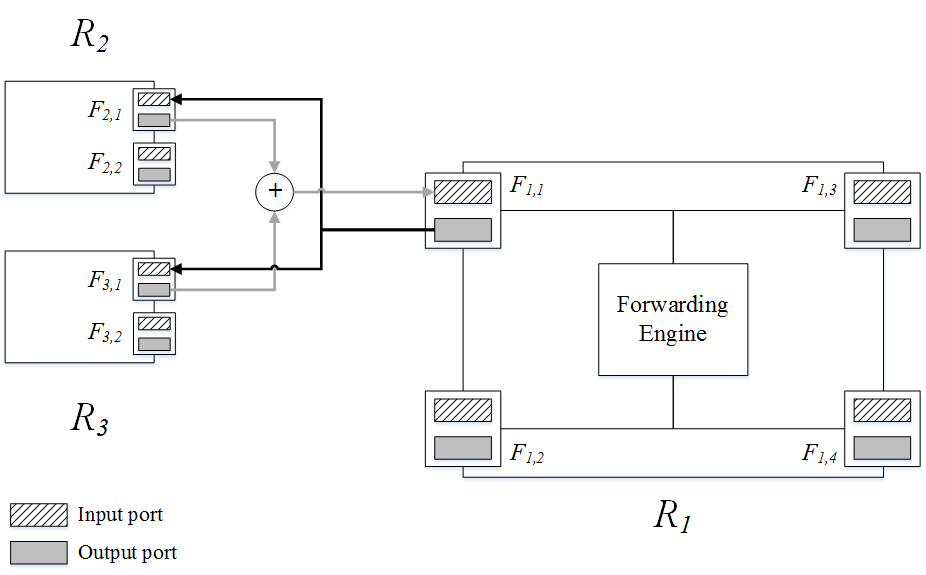
\includegraphics[width=0.40\textwidth]{figures/ndn-router-overview.png}
    \cprotect\caption{Graphical depiction of our NDN router model.}
    \label{fig:ndn-router-overview}

\end{figure}

Figure~\ref{fig:ndn-router-overview} provides a graphical description of the proposed 
router model. A router $R$ contains a set of $|F|$ interfaces $F$, used to interconnect 
it to other entities (e.g. some other router $R'$, a client $C$ or the server 
$S$). Each interface can subsequently be divided into one input and one output 
port, which `cross-connect' with the ports of the attached 
interfaces (see Figure~\ref{fig:ndn-router-overview}). We use the notation 
$F_{r,f,in}$ or $F_{r,f,out}$, to refer to the 
input\slash output ports of an interface $f$, of a router $R_r$.\shortvertbreak

The act of forwarding some set of Interest\slash Data packets from a router $R_1$, 
over some interface $F_1$, is modeled by having $R_1$ fill $F_{1,1,out}$ with 
some set of signals \textbf{u}, following the encoding shown in 
Section~\ref{subsec:meth-overview}. Conversely, the act of receiving some set 
of Interest\slash Data packets is modeled by having routers $R_2$ and $R_3$ --- 
connected with $F_{1,1}$ via $F_{2,1}$ and $F_{3,1}$ --- fill $F_{2,1,in}$ and $F_{3,1,in}$ 
with \textbf{u} \footnote{In fact, this procedure can be extended to any network entity, let 
it be a router, a client or the server.}. As seen in Figure~\ref{fig:ndn-router-overview}, 
more than one entity may be connected to some interface, in which case the 
signals \textbf{u} originating from the interconnected interfaces' output ports, 
e.g. $F_{2,1,out}$ and $F_{3,1,out}$, are combined and summed at the other 
end's input port, e.g. $F_{1,1,in}$. While the use of interfaces and 
input\slash output ports may be seen as a case of over engineering, we argue 
it makes our model robust, highly modular and capable of supporting multiple 
network topologies.\shortvertbreak

\subsubsection{Pending Interest Table (PIT)}
\label{subsec:meth-pit}

In the same way that the FIB commands the forwarding of Interests, the PIT 
commands the forwarding of Data packets. Nevertheless, the composition of the 
PIT is more dynamic than that of the FIB, being dependent on the flow of 
Interest and Data packets through the NDN router.\shortvertbreak

Similarly to the FIB, we model the PIT as a $|O| \times |F|$ matrix in the 
form

\begin{equation}
\textbf{PIT} = \begin{bmatrix} 1 & 0 & 0 & 0  \\ 
                1 & 0 & 0 & 0               \\ 
                0 & 1 & 0 & 0               \\ 
                0 & 1 & 0 & 0               \\ \end{bmatrix}
    \label{eq:pit}
\end{equation}\shortvertbreak

\textbf{PIT}\footnote{We use the form `PIT' for general references to the Pending 
Interest Table, and `\textbf{PIT}' when referring to its matrix form, as in~\ref{eq:pit}. 
This dual representation is extended to the FIB and CS.} entries 
$(o,f)$ are encoded as 0 or 1: if $(o,f) = 1$, that means that Data 
packets of 
type $O_o$ have been previously requested via interface $F_f$, and so Data 
packets $d_{O_o}$ shall be forwarded via $F_f$; on the other hand, 
if $(o,f) = 0$, $d_{O_o}$ should not be forwarded via that 
interface. These operations influence the composition of the \textbf{PIT} over time, whose 
maintenance can be summarized by the two simple routines shown below, to be 
followed upon Interest and Data packet arrivals, respectively. For the algorithms shown 
below, we consider a special matrix \textbf{A}, corresponding to the concatenation of 
all the arrays $\textbf{u}_{r,f,in}$ as columns, i.e. the contents from the input ports 
of all the interfaces $F_f$, at some router $R_r$:

\begin{equation}
\textbf{A} = \begin{bmatrix} \textbf{u}_{r,1,in} & \textbf{u}_{r,2,in} & ... & \textbf{u}_{r,|F|,in} \end{bmatrix}
    \label{eq:a}
\end{equation}\shortvertbreak

\begin{algorithmic}[1]

\State \textbf{define} updateOnInterest(\textbf{A}):
\State
    \State $\textbf{A}' \leftarrow \textbf{A}(1:|O|,:)$
    \State $\textbf{D} \leftarrow$ diag$(\neg(\textbf{PIT} \times \textbf{1}))$
    \State $\textbf{B} \leftarrow \textbf{D} \times \textbf{A}'$ 
    \State \textbf{PIT} $\leftarrow$ \textbf{PIT} $|$ $\textbf{A}'$ 
    \State \Return $\textbf{B}$

\end{algorithmic}\shortvertbreak

Upon the reception of Interest signals, i.e. $\textbf{A}'$ (the first $|O|$ rows 
of $\textbf{A}$), we first identify the content items $O_o$, or the rows indexes of the 
\textbf{PIT}, for which there are \textbf{no} pending Interests, in line 4. For 
convenience, we often recur to binary operations (negation `$\neg$', 
conjunction `$\&$', disjunction `$|$') over matrices: e.g. in line 4, after 
summing all columns of the \textbf{PIT}\footnote{We use the notation \textbf{1} for the 
sum vector, i.e. $\textbf{1} = [1\,1\,...\,1]^{T}$.}, we negate the 
result, obtaining a binary encoded $|O| \times 1$ 
column vector which indicates the absence (encoded as  `1') and presence 
(encoded as `0') of pending Interests for some content object $O_o$. We diagonalize 
the result, so that it is appropriate for multiplication with $\textbf{A}'$. In line 5, 
we 
keep the rows of $\textbf{A}'$ with such indexes, `erasing' the remaining rows (i.e. 
setting their elements to 0). These are saved in $\textbf{B}$, which consist in the only 
Interest signals that the NDN router needs to forward upstream. Note that even 
if $\textbf{A}'$ includes some $i_{O_o} > 1$, we only need to forward one Interest 
over the interfaces specified in the FIB, and so the binary encoding of $\textbf{B}$, 
resulting from the use of binary operations, neatly serves our purposes. 
In line 6, the 
contents of the \textbf{PIT} are updated by performing a logic OR, `$|$', with $\textbf{A}'$, so 
that it registers all the newly received 
Interest signals and their correspondence to interfaces. This last step is important, 
as it allows future Data packets to be forwarded downstream over the requesting 
interfaces.\shortvertbreak

\begin{algorithmic}[1]

\State \textbf{define} updateOnData($\textbf{A}$):
\State
    \State $\textbf{A}' \leftarrow \textbf{A}(|O|+1:2\,|O|,:)$
    \State $\textbf{D} \leftarrow \textbf{A}' \times \textbf{1}$
    \State $\textbf{E} \leftarrow$ diag$(\textbf{D}) \times$ \textbf{PIT}
    \State \textbf{PIT} $\leftarrow$ diag$(\neg\,\textbf{D}) \times$ \textbf{PIT}
    \State \Return $\textbf{E}$

\end{algorithmic}\shortvertbreak

With the explanation given above for the \textbf{updateOnInterest()} routine, 
the understanding of \textbf{updateOnData()} is left to the reader. Note that 
the objective of this last routine is the reverse operation of \textbf{updateOnInterest()}, i.e. forwarding Data 
packets over the interfaces for which there is a registered Interest in the \textbf{PIT}. We 
also note that the final step of the operation (line 6) consists in erasing 
all Interest registrations which have been successfully attended.\shortvertbreak

\subsubsection{Forwarding Information Base (FIB)}
\label{subsec:meth-fib}

The FIB is important for the act of forwarding Interest packets towards 
appropriate content sources, by indicating the interfaces $F$ over which such 
sources are reachable. For each NDN router $R$, we model the FIB as a simple 
$|O| \times |F|$ matrix in the form

\begin{equation}
\textbf{FIB} = \begin{bmatrix} 1 & 0 & 0 & 0  \\ 
                1 & 0 & 0 & 0               \\ 
                0 & 1 & 0 & 0               \\ 
                0 & 1 & 0 & 0               \\ \end{bmatrix}
    \label{eq:fib}
\end{equation}\shortvertbreak

The \textbf{FIB} encoding shown in~\ref{eq:fib} would be held by router $R_1$ in the 
simple topology shown in Figure~\ref{fig:fib-topo}. \textbf{FIB} entries 
$(o,f)$ are encoded as 0 or 1: if $(o,f) = 1$, content objects of 
type $O_o$ are accessible via interface $F_f$, meaning that Interests 
$i_{O_o}$ shall be forwarded via $F_f$; on the other hand, 
if $(o,f) = 0$, $i_{O_o}$ should not be forwarded via that interface. 
Following the same type of operations described for the PIT 
in Section~\ref{subsec:meth-pit}, we now present the algorithm followed by NDN 
routers to forward the Interest signals, $\textbf{B}$, returned by the 
\textbf{updateOnInterest()} operation:\shortvertbreak 

\begin{algorithmic}[1]

\State \textbf{define} forwardData($\textbf{B}$):
\State
    \State $\textbf{B}' \leftarrow \textbf{B} \times \textbf{1}$
    \State $\textbf{L} \leftarrow$ diag$(\textbf{B}) \times$ \textbf{FIB}
    \State $F_{n,1:|F|,out} \leftarrow \textbf{L}$

\end{algorithmic}\shortvertbreak

The last operation of the \textbf{forwardData()} routine (line 5) refers to 
the (parallelized) `filling' of the output ports of all the interfaces $F$ of router $R_r$.\shortvertbreak

In our model, the composition of the \textbf{FIB} is established at an initial phase, 
not suffering any further alterations (more details in 
Section~\ref{subsec:meth-conn-dots}). Note 
that the FIB only commands Interest forwarding actions, not participating in the 
forwarding of Data packets.\shortvertbreak

\begin{figure}[h!]

    \centering
    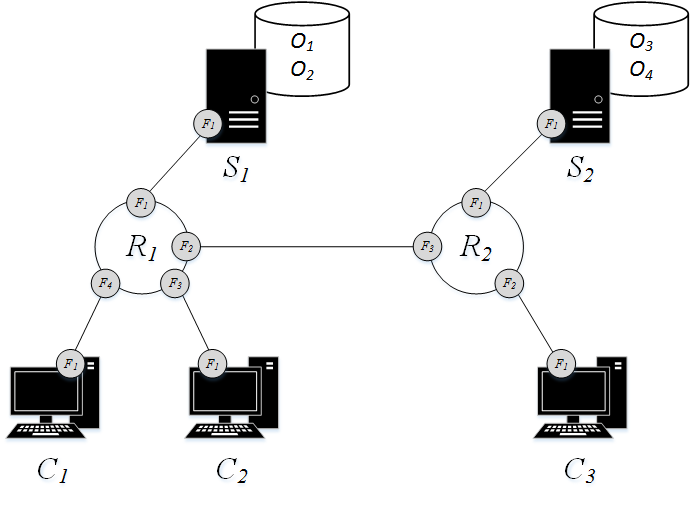
\includegraphics[width=0.40\textwidth]{figures/fib-topo.png}
    \cprotect\caption{Simple example of an NDN network topology.}
    \label{fig:fib-topo}

\end{figure}

\subsubsection{Content Store (CS)}
\label{subsec:meth-cs}

We model the Content Store (CS), i.e. the NDN router's cache, as an $|O| 
\times |P|$ matrix, in which $|P|$ is the size of the CS, i.e. maximum 
number of content objects it is able to accommodate at any given point in time. 
We use $P$ to represent a position or slot in the CS, which is able to hold a single 
content object $O_o$ (here we do not consider a notion of content object size, 
an object always fits in a slot $P$). E.g. in~\ref{eq:cs} we show the encoding 
of the \textbf{CS} for $R_1$ in Figure~\ref{fig:fib-topo}, with $|P| = 2$, 
which is shown to contain content objects $O_2$ and $O_4$\footnote{Usually, 
we consider $|P| << |O|$.}.

\begin{equation}
\textbf{CS} = \begin{bmatrix} 0 & 0             \\ 
                1 & 0                           \\ 
                0 & 1                           \\ 
                0 & 0                           \\ \end{bmatrix}
    \label{eq:cs}
\end{equation}\shortvertbreak

Again, we follow a binary encoding, using $(o, p) = 1$ to indicate the 
presence of content $O_o$ at slot $P_p$, and $(o, p) = 0$ as an indication of 
its absence. Each slot is assigned a different integer 
index, i.e. $P_p$, with $p = \{1, 2, ..., |P|\}$, which express the idea of `levels': 
$O_o$, occupying slot $P_2$, is at the 2\textsuperscript{nd} 
(highest) position of the \textbf{CS}. $P_1$ is usually interpreted as the `highest' 
level, and $P_{|P|}$ the `lowest', nevertheless the meaning is of the `levels' 
is often dependent on the caching algorithm implemented by the CS. In fact, we 
model a CS as having a general behavior (presented in this section), and a specific 
behavior, which depends on the cache algorithm the CS implements. We discuss caching 
algorithms in Section~\ref{subsec:meth-caching-algs}.\shortvertbreak

Note that \textbf{CS} must obey a set of constraints, since (1) 
each slot can only hold a single content object, and (2) it is inefficient for 
the \textbf{CS} to hold multiple copies of a content $O_o$. Specifically, the 
conditions for the validity of \textbf{CS} are:

\begin{equation}
    \sum_{o=1}^{|O|} \textbf{CS}_{o,p} \le 1 \quad \forall \ p \in {1, 2, ..., |P|}
    \label{eq:cs-constraints-1}
\end{equation}

\begin{equation}
    \sum_{p=1}^{|P|} \textbf{CS}_{o,p} \le 1 \quad \forall \ o \in {1, 2, ..., |O|}
    \label{eq:cs-constraints-2}
\end{equation}\shortvertbreak

\subsection{Endpoints}
\label{subsec:meth-endpoints}

\subsection{Caching Algorithms}
\label{subsec:meth-caching-algs}

\subsection{`Connecting the Dots'}
\label{subsec:meth-conn-dots}

We represent a network topology using a square matrix \textbf{T}, 
with dimension $|R|+|C|+|S|$. For representation purposes, we attribute an 
integer index to each one of the network nodes, and so each elements $(i,j)$ of the 
matrix corresponds to interconnections between network entities with indexes $i$ and $j$. The 
values at each $(i,j)$ position identify the \textbf{near end interface} of the 
connection, i.e. the interface at entity $i$. E.g. the matrix \textbf{T} shown 
in~\ref{eq:topo} encodes the topology shown in Figure~\ref{fig:fib-topo}. In this case, 
we attribute the integers 1 to 7 to the network entities, starting with the 
clients $C_1$ to $C_3$, then routers $R_1$ and $R_2$ and 
finally the servers $S_1$ and $S_2$.

\begin{equation}
\textbf{T} = \begin{bmatrix} 
                0 & 0 & 0 & 1 & 0 & 0 & 0               \\ 
                0 & 0 & 0 & 1 & 0 & 0 & 0               \\ 
                0 & 0 & 0 & 0 & 1 & 0 & 0               \\ 
                4 & 3 & 0 & 0 & 2 & 1 & 0               \\ 
                0 & 0 & 2 & 3 & 0 & 0 & 1               \\ 
                0 & 0 & 0 & 1 & 0 & 0 & 0               \\ 
                0 & 0 & 0 & 0 & 1 & 0 & 0               \\ \end{bmatrix}
    \label{eq:topo}
\end{equation}\shortvertbreak


